\documentclass[12pt, a4paper, twoside]{book}
\usepackage[utf8]{inputenc} % Aceptar diferentes tipos de codificación de caracteres de entrada (en este caso usamos la codificación Unicode UTF-8)
%\usepackage{natbib}
\usepackage{listings}
\usepackage{eurosym}
\usepackage[spanish]{babel}
\usepackage{titlesec}
\usepackage{graphicx} % Soporte aumentado para gráficos 
\usepackage{float}
\usepackage{hyperref} % Para manejar referencias cruzadas. P.ej. añadir hiperenlaces al índice
\usepackage{caption}
\usepackage{setspace}
\usepackage{color}
\usepackage[a4paper, top=3.5cm, bottom=3.5cm, left=3cm, right=3cm]{geometry}
\spacing{1.5}
\setcounter{secnumdepth}{4}
\setlength{\parindent}{12pt}
\titleformat{\paragraph}
{\normalfont\normalsize\bfseries}{\theparagraph}{1em}{}
\titlespacing*{\paragraph}
{0pt}{3.25ex plus 1ex minus .2ex}{1.5ex plus .2ex}

%\usepackage{inconsolata}
%
%\usepackage[T1]{fontenc}
%
%\definecolor{pblue}{rgb}{0.13,0.13,1}
%\definecolor{pgreen}{rgb}{0,0.5,0}
%\definecolor{pred}{rgb}{0.9,0,0}
%\definecolor{pgrey}{rgb}{0.46,0.45,0.48}
%
%\lstset{language=Java,
%	showspaces=false,
%	showtabs=false,
%	breaklines=true,
%	showstringspaces=false,
%	breakatwhitespace=true,
%	commentstyle=\color{pgreen},
%	keywordstyle=\color{pblue},
%	stringstyle=\color{pred},
%	basicstyle=\ttfamily,
%	moredelim=[il][\textcolor{pgrey}]{$$},
%	moredelim=[is][\textolor{pgrey}]{\%\%}{\%%}
%}


\begin{document}	
	
	\thispagestyle{empty} 	
	%%%%%%%%%%%%%%%%%%%%%%%%%%%%%%%%%%%%%%%%%%%%%%%%%%%%%%%%%%%%%%%%%%%%%%%%%%%%%%%%
	% PORTADA
	%%%%%%%%%%%%%%%%%%%%%%%%%%%%%%%%%%%%%%%%%%%%%%%%%%%%%%%%%%%%%%%%%%%%%%%%%%%%%%%%
	
	\begin{center}		
		
\includegraphics[width=15cm]{Imagenes/Simbolo_logo_UDC.png}
	\end{center}
	
	% Lista de tamaños: \Huge, \huge, \LARGE, \Large, \large, \small, \footnotesize, \tiny
	\vspace{2cm}
	
	\begin{center}		
		{\textbf{ FACULTADE DE INFORMÁTICA}}
		
		\vspace{1cm}
		\LARGE{ TRABALLO FIN DE MÁSTER }	\\
		\LARGE{ MÁSTER UNIVERSITARIO EN INGENIERÍA INFORMÁTICA } \\
		\vspace{1cm}	
		\LARGE{\textbf{ Aplicación web para a xestión de menús domésticos con servizos nutricionais : Eat Fit Week! }}
	\end{center}
	
	\vspace{2cm}
	\hfill \textbf{Autor: \textit{Elías Ferreiro Borreiros}}
	
	
	\hfill \textbf{Director: \textit{Juan José Sánchez Penas}} 
	
	
	\hfill A Coruña, Agosto, 2019					
	
	\clearpage
	
	\begin{center}
		\LARGE{\textbf{ RESUMEN }}	
	\end{center}
	Hoy en día, con el cambio en los estilos de vida de las personas y tendiendo hacia unas costumbres más sedentarias, hay una mayor necesidad de enfocarse en una dieta equilibrada y saludable.
	Para ello, se han desarrollado muchos sistemas webs y móviles para la gestión de comidas y de sus valores nutricionales.	Sin embargo, analizando esos sistemas, vemos que tienen un error en su planteamiento al inundar a los usuarios con formularios sobrecargados y repletos de información innecesaria. 
	El otro problema principal de estos sistemas es la cantidad exagerada de trabajo manual que debe hacer el usuario antes de poder disfrutar de la funcionalidad principal. 
	
	Para resolver todo esto, hemos decidido plantear el desarrollo de una aplicación que solvente estos problemas y ofrezca una funcionalidad que no disponen los competidores : el análisis nutricional dinámico de las comidas planificadas para la semana configurable por el usuario. está sobrepasando.
	
	A mayores permitiremos la gestión de las entidades necesarias para esta planificación: ingredientes, platos, menús ... 
	Esto se hará siguiendo la filosofía inicial del proyecto: simplificar la entrada lo más posible y disminuir el esfuerzo requerido por el usuario. 
	Para esto llamaremos a servicios externos que nos permitirán estimar las características nutricionales de los ingredientes de forma que el usuario no tendrá que indicar esos datos y permitiremos con cada registro de usuario el alta automática de unos ingredientes base utilizables en la mayoría de recetas que agilizarán la configuración necesaria de un nuevo perfil para permitir disfrutar al máximo al usuario de las funcionalidades realmente importantes desde el momento más temprano posible.
	
	\clearpage
	
	\textbf{Título:} Aplicación web para a xestión de menús domésticos con servizos nutricionais
	\\
	\textbf{Autor:} Elías Ferreiro Borreiros
	\\
	\textbf{Tutor/Director:} Juan José Sánchez Penas
	
	
	\textbf{Palabras clave:} Java EE, POJO, Maven, Angular JS, Spring, Hibernate, Web, MySQL, Tarea, Lista, Contexto, Cliente - Servidor, Food, Planning, Management, Scrum. 
	
	
	\renewcommand{\contentsname}{Índice de contenidos}
	\renewcommand{\listfigurename}{Índice de figuras}
	\renewcommand{\listtablename}{Índice de tablas}
	
	\tableofcontents % indice de contenidos
	
	\listoffigures % indice de figuras
	
	\listoftables % indice de tablas
	
	\clearpage
	
	\chapter{INTRODUCCIÓN AL DESARROLLO REALIZADO}
	\section{Metodología e Iteraciones}
	Para que un proyecto software se realice correctamente es necesario seguir una metodología adecuada a su tamaño y propósito. La metodología utilizada para desarrollar este proyecto ha sido Scrum.
	\subsection{Scrum}
	Scrum es un marco de trabajo para desarrollo ágil de software.\\
	Es un proceso en el que se aplican de manera regular un conjunto de buenas prácticas para trabajar colaborativamente, en equipo y obtener el mejor resultado posible de proyectos, caracterizado por:
	\begin{itemize}
		\item Adoptar una estrategia de desarrollo incremental, en lugar de la planificación y ejecución completa del producto.
		\item Basar la calidad del resultado más en el conocimiento tácito de las personas en equipos auto organizados, que en la calidad de los procesos empleados.
		\item Solapar las diferentes fases del desarrollo, en lugar de realizar una tras otra en un ciclo secuencial o en cascada.
	\end{itemize}	
	\begin{figure}[H]
		\centering
		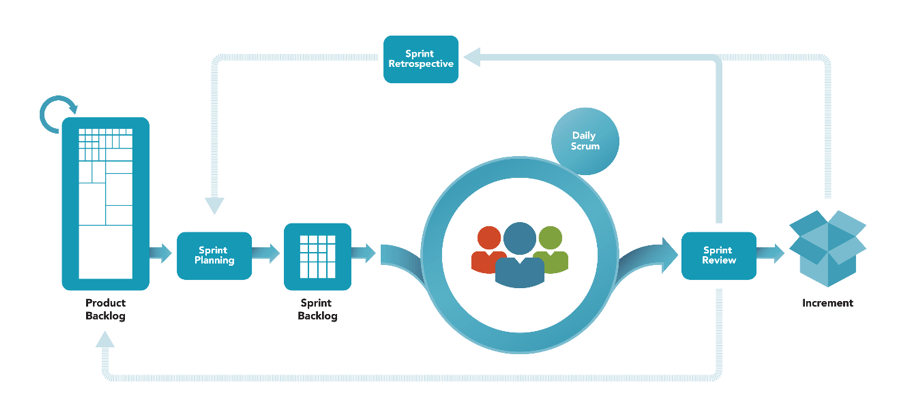
\includegraphics[width=15cm]{Imagenes/Scrum.png}
		\caption{Scrum}\label{Scrum}
	\end{figure}
	Se toma la decisión de esta metodología ya que con el desarrollo iterativo nos permitirá adaptarnos a los posibles cambios de alcance que se encuentren en el desarrollo del proyecto. También nos permitirá hacer un seguimiento muy cercano al avance del proyecto permitiéndonos corregir el enfoque en caso de estarnos desviando del camino correcto.
	\chapter{PLANIFICACIÓN Y ANÁLISIS DE COSTES}
	\section{Análisis de viabilidad}
	Ya que vemos que existen muchos otros sistemas similares al nuestro, realizamos encuestas con diferentes potenciales usuarios de nuestro sistema y les explicamos el enfoque que diferenciaría al nuestro y que supone una ventaja con respecto al resto, el seguimiento de los stats nutricionales de los menús semanales y el diseño minimalista y user friendly de nuestras interfaces. Tras recibir resultados positivos de todas las personas con las que hemos hablado, realizamos una planificación del trabajo necesario para implementar el sistema para poder estimar el esfuerzo requerido y ver si sería una cantidad manejable.
	\section{Planificación}
	El objetivo de la división del trabajo es poder organizar estas tareas en Sprints.\\
	Sprint es el nombre que va a recibir cada uno de los ciclos o iteraciones que vamos a tener dentro de dentro de nuestro proyecto.\\	
	Nos van a permitir tener un ritmo de trabajo con un tiempo prefijado, siendo la duración de nuestro Sprint una semana. Teniendo sprints cortos tenemos una mayor adaptabilidad al cambio y un seguimiento más cercano del avance.	En cada Sprint o cada ciclo de trabajo lo que vamos a conseguir es lo que se denomina un entregable o incremento del producto, que aporte valor al cliente.
	En esta división obtenemos la siguiente lista de historias de usuario ordenadas por prioridad, descripción de una funcionalidad que debe incorporar un sistema de software, y cuya implementación aporta valor al cliente:
	\begin{itemize}
		\item HU01-Dar de alta un ingrediente
		\item HU02-Dar de alta un plato
		\item HU03-Visión semanal de menú
		\item HU04-Generación de lista de la compra
		\item HU05-Gestión de usuarios
		\item HU06-Configuraciones de usuario: dietéticas y de preferencias
		\item HU07-Análisis dietético dinámico de menú
		\item HU08-Integración con WS de características nutricionales para estimación de ingredientes
		\item HU09-Integración con supermercados para estimar un precio de la compra
		\item HU10-Recetario
		\item HU11-Generación aleatoria de menú
		\item HU12-Generación de menú de acorde a las características dietéticas
		\item HU13-Compartición por redes sociales
		\item HU14-Énfasis en UX y diferentes tamaños de pantalla
		\item HU15-Machine Learning para sugerir platos nuevos
	\end{itemize}
	\subsection{Planificación previa}
	Este proyecto cuenta principalmente con dos recursos, un Analista/Programador que es el creador de esta memoria, y un Jefe de Proyecto que es el director del mismo Juan José Sánchez. Para ambos recursos un día de trabajo consta de 8 horas.
	\subsection{Sprints}
	Realizaremos el desarrollo del proyecto en 10 semanas con lo que tendremos 10 sprints. Realizamos la asignación de las historias de usuario a cada uno de los sprints balanceándolas de forma que todos los sprints tengan la misma carga de trabajo:
	\begin{itemize}
		\item Sprint 1 : HU01-Dar de alta un ingrediente y HU02-Dar de alta un plato
		\item Sprint 2 : HU03-Visión semanal de menú
		\item Sprint 3 : HU04-Generación de lista de la compra
		\item Sprint 4 : HU05-Gestión de usuarios y HU06-Configuraciones de usuario: dietéticas y de preferencias
		\item Sprint 5 : HU07-Análisis dietético dinámico de menú
		\item Sprint 6 : HU08-Integración con WS de características nutricionales para estimación de ingredientes
		\item Sprint 7 : HU09-Integración con supermercados para estimar un precio de la compra
		\item Sprint 8 : HU10-Recetario
		\item Sprint 9 : HU11-Generación aleatoria de menú y HU12-Generación de menú de acorde a las características dietéticas y HU13-Compartición por redes sociales
		\item Sprint 10 : HU14-Énfasis en UX y diferentes tamaños de pantalla y HU15-Machine Learning para sugerir platos nuevos
	\end{itemize}
	
	
	\begin{tabular}{| p{5cm} | p{3cm} | p{3cm} | p{3cm} |}
		\hline
		\textbf{Recurso} & \textbf{Nome} & \textbf{Coste/hora} & \textbf{Coste/día}
		\\ \hline
		{Analista/Programador} & {Elías Ferreiro Borreiros} & {30\euro} & {240\euro}
		\\ \hline
		{Jefe de Proyecto} & {Juan José Sánchez} & {50\euro} & {400\euro}
		\\ \hline
		
	\end{tabular}		
	
	\captionof{table}{Recursos empleados en el proyecto}
	
	\begin{tabular}{|p{5cm} | p{2cm} | p{2cm} | p{2cm} | p{2cm} |}
		
		\hline
		\textbf{Recurso} & \textbf{Sprints} & \textbf{Horas / Sprint} & \textbf{Coste / Sprint} & \textbf{Coste total (\euro)}
		\\ \hline
		\textbf{Analista/Programador} & 10 & 40 & 1200\euro  & 12000\euro
		\\ \hline
		\textbf{Xefe de Proxecto} & 10 & 40 & 2000\euro & 20000\euro		
		\\ \hline
		\textbf{TOTAL} & & & & 212000\euro
		\\ \hline
	\end{tabular}
	
	\captionof{table}{Costes totales siguiendo la planificación}
	
\end{document}

